\section{Windshield Wiper Model}
As Fig.5 shows,  the windshield wiper model is consisted of an expression and a multiplier. If the wiper is OFF, the expression outputs 1 to the multiplier, which means no water is wiped out; if the wiper works in SLOW mode, the expression outputs 0.5 to the multiplier, which means 50\% water is wiped out; if the wiper works in FAST mode, the expression outputs 0.2 to the multiplier, which means 80\% water is wiped out.

\begin{center}
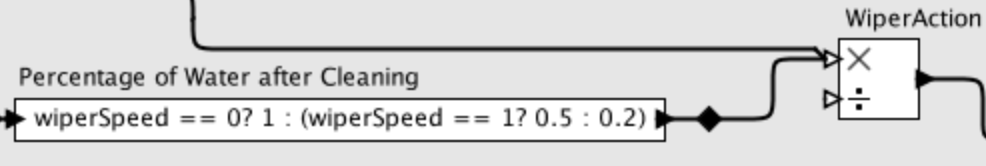
\includegraphics[width=13.5cm]{fig5.png}
\end{center}
\begin{center}
\small{Figure 5. The Windshield Wiper Model}
\label{wiper}
\end{center}